\documentclass[11pt]{article}

\usepackage[a4paper,margin=2.6cm]{geometry}
\usepackage[T1]{fontenc}
\usepackage[utf8]{inputenc}
\usepackage{lmodern}
\usepackage{microtype}
\usepackage{amsmath,amssymb,amsthm}
\usepackage{booktabs}
\usepackage{graphicx}
\usepackage{xcolor}
\usepackage[font=small,labelfont=bf]{caption}
\usepackage{enumitem}
\definecolor{linkblue}{HTML}{1c5cab}
\usepackage[colorlinks=true,linkcolor=linkblue,citecolor=linkblue,urlcolor=linkblue]{hyperref}

\newtheorem{proposition}{Proposition}
\newcommand{\sillage}{\textsc{Sillage}}
\newcommand{\dnll}{\Delta\mathrm{NLL}}
\newcommand{\ci}[2]{{\footnotesize[#1,\,#2]}}

\title{\bfseries \textsc{Sillage}: Surprise-Gated Amplitude Memory\\
for Frozen Language Models}
\author{Abderrahmane Sghairi\\
\small Independent Researcher, Issoire, France\\
\small \texttt{sghairipro63@gmail.com}}
\date{August 2026\\[2pt]
\small DOI: \href{https://doi.org/10.5281/zenodo.22079016}{10.5281/zenodo.22079016}
\qquad Code: \href{https://github.com/riscoss63/sillage}{github.com/riscoss63/sillage}}

\begin{document}
\maketitle

\begin{abstract}
We augment frozen language models with a \emph{fixed-size} Hebbian associative memory that adapts at inference time with no gradients, no backpropagation, and no growth in storage. The memory is a single matrix ($4.2$\,MB). Keys are sliding $n$-gram bindings of random token hypervectors, whose retrieval kernel is near-orthogonal except under exact repetition; values are token hypervectors whose stored coefficients are maintained as \emph{amplitudes} --- square roots of accumulated mass --- by a local read-modify-write rule inspired by the classical square-root (Bhattacharyya) embedding of probability distributions; and every write is gated by the model's own token surprise $-\ln p_{\mathrm{LM}}$, a three-factor plasticity rule whose modulator is free at inference. We call the system \sillage{}. On a 36k-token stream of novel technical text, the memory improves GPT-2's test negative log-likelihood by $+0.486 \pm 0.005$ nats (perplexity $31.2 \to 19.2$; mean$\,\pm\,$SEM over 5 hypervector seeds), \textbf{outperforming an unbounded kNN-LM ($+0.281$; paired block-bootstrap $P=1.000$) with $13\times$ less memory}, an exact $n$-gram cache ($+0.318$), a byte-matched kNN-LM ($+0.174$), and retrieval-augmented rescoring ($+0.043$). On a second, modern model (Qwen3-0.6B) the mechanism orderings replicate and \sillage{} statistically matches unbounded kNN-LM at one-sixteenth the memory; on a downstream content-token recall task, the augmented models complete recurring technical terms at up to $2.1\times$ the frozen model's accuracy after a single reading pass. Ablations attribute the gain: amplitude encoding contributes $+0.28$ nats over count encoding (the largest single factor; $P=1.000$ in every seed), surprise gating quadruples the gain of uniform writes, and a multi-scale key doubles gains on low-repetition text. At 500k tokens the fixed matrix saturates ($0.5$ writes per parameter); leaky decay recovers $2.3\times$ of the gain and a $4\times$ larger matrix recovers $3.4\times$, quantifying a capacity-sizing law, while unbounded kNN-LM (grown to 770\,MB) dominates on long narrative --- an honestly mapped regime boundary. Two evaluation artifacts (a corpus-formatting pathology producing $+1.35$ nats of phantom gains, caught by a shuffled-retrieval control; an off-by-one in the RAG baseline) are documented so others avoid them. Code and data scripts are released.
\end{abstract}

\section{Introduction}

Large language models are frozen at deployment: they neither remember what they have just read nor adapt to the document in front of them, unless one pays for fine-tuning, a growing retrieval index, or long-context attention. The non-parametric remedy --- kNN-LM \cite{khandelwal2020} and its descendants --- interpolates the model's prediction with retrieval from a datastore of (hidden state, next token) pairs; but the datastore grows linearly with everything read, and each query scans it. Recent \emph{test-time memorization} architectures --- Titans \cite{titans}, test-time-training layers \cite{ttt}, and the unifying test-time-regression view \cite{ttr} --- learn a bounded neural memory during inference, but update it with gradient-based rules.

This paper asks how far one can get with the \emph{oldest} memory mechanism --- a single Hebbian outer-product matrix, written once per token and never trained --- provided three design choices are made correctly:

\begin{enumerate}[leftmargin=1.4em,itemsep=2pt]
\item \textbf{What is a key?} Not the LM's hidden state: we show its similarity geometry is too entangled for a linear Hebbian readout (a measured negative result, Appendix~\ref{app:negative}). Instead, a \emph{compositional $n$-gram binding} of token hypervectors, computed by a sliding vector-symbolic product, whose kernel is a near-delta on exact repetition (Proposition~\ref{prop:kernel}).
\item \textbf{What is a value coefficient?} Not a count. We maintain \emph{amplitudes} --- square roots of accumulated mass --- with a local read-modify-write update. This adapts the classical square-root embedding of probability vectors \cite{bhatta43,rootsift,jebara} to a superposed memory: square-root compression bounds the dynamic range of coefficients, so frequent successors no longer drown rare ones in crosstalk (Proposition~\ref{prop:amp}). It is the largest single contributor to performance.
\item \textbf{When to write?} Proportionally to \emph{surprise}. The modulator of this three-factor rule \cite{fremaux,izhikevich} is the model's own token log-loss --- available for free at inference --- or, better, the surprise of the augmented system (LM $+$ memory), which stops the memory from over-writing what it already predicts.
\end{enumerate}

The resulting system --- \sillage{}\footnote{\emph{Sillage} (French): the trace left behind by something that has passed --- a ship's wake, a scent in a room. What the memory keeps of what the model read.}, a surprise-gated amplitude memory --- is a 4.2\,MB matrix with $O(1)$ storage, one matrix--vector read and one rank-1 write per token, no gradients anywhere, and a direct biological reading: Hebbian synapses under neuromodulatory gain control.

\paragraph{Contributions.}
\textbf{(C1)} A fixed-size, gradient-free memory that beats unbounded kNN-LM on novel repetitive text (paired $P=1.000$) at $1/13$th the memory, and beats retrieval-augmented rescoring and an exact $n$-gram dictionary on the same stream (\S\ref{sec:main}); the result replicates on a second, modern LM (\S\ref{sec:qwen}).
\textbf{(C2)} A downstream evaluation: content-token recall after one reading pass, where the augmented model completes recurring technical terms far more accurately than the frozen model (\S\ref{sec:cloze}).
\textbf{(C3)} A factorial attribution of the gain to its three mechanisms, replicated over 5 hypervector seeds with every effect positive in every seed (\S\ref{sec:mech}).
\textbf{(C4)} A scaling study to 500k tokens that maps the honest regime boundary --- saturation at $\sim$0.5 writes/parameter, a $2.3\times$ recovery from leaky forgetting, a $3.4\times$ recovery from $4\times$ capacity, and the persisting advantage of unbounded retrieval on long narrative (\S\ref{sec:scaling}).
\textbf{(C5)} A measured negative result (frozen-LM hidden states are unusable as Hebbian keys) and two documented evaluation artifacts with the controls that caught them (\S\ref{sec:integrity}), offered as methodology for streaming-memory evaluations.

\section{Related work}

\textbf{Non-parametric LM augmentation.} kNN-LM \cite{khandelwal2020} interpolates the LM with retrieval over exact hidden-state keys; the continuous cache \cite{grave} is its local ancestor; RETRO \cite{retro} and Memorizing Transformers \cite{memtrans} move retrieval inside the architecture. All maintain stores that grow with the data; \sillage{} targets the same interpolation interface with a store of constant size.

\textbf{Test-time memorization.} Titans \cite{titans} learns a neural long-term memory at inference, gated by a \emph{gradient-based} surprise signal with momentum and adaptive forgetting; test-time-training layers \cite{ttt} make the hidden state a set of learned weights; test-time regression \cite{ttr} unifies these designs as associative memories, and nested learning \cite{nested} generalizes the multi-timescale view. \sillage{} occupies the gradient-free corner of this space: its surprise is the log-loss the LM computes anyway, its update is a rank-1 Hebbian write, and its forgetting is a scalar leak --- while reproducing the same qualitative ingredients (surprise gating, decay) that these systems learn. Modern Hopfield theory \cite{hopfield} connects attention itself to associative retrieval.

\textbf{Vector symbolic architectures.} Hypervector binding, superposition and cleanup \cite{kanerva,plate,kleyko} provide the key/value algebra; our sliding $n$-gram key is a permuted binding with an incremental exact-window update. The square-root encoding of nonnegative vectors is classical --- the Bhattacharyya affinity \cite{bhatta43}, probability-product kernels \cite{jebara}, and Hellinger (``RootSIFT'') normalization in vision \cite{rootsift} --- and Section~\ref{sec:values} adapts it to superposed Hebbian storage.

\textbf{Three-factor plasticity.} Neuromodulated Hebbian rules gate synaptic change by a global scalar \cite{fremaux,izhikevich}; \sillage's scalar is the free-energy signal of the (augmented) model itself.

\section{Method}\label{sec:method}

\begin{figure}[t]
\centering
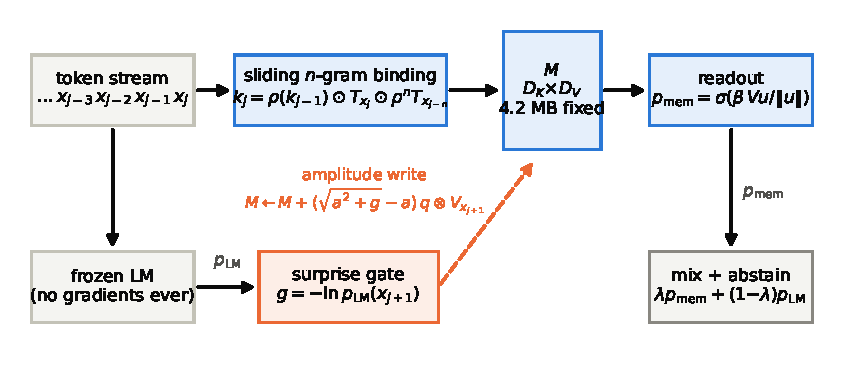
\includegraphics[width=0.92\linewidth]{figs/fig0_architecture.pdf}
\caption{The \sillage{} loop. Read path (blue): a sliding $n$-gram binding of token hypervectors addresses a fixed matrix $M$; the retrieved vector is scored over the vocabulary and mixed with the frozen LM. Write path (orange, dashed): the LM's own token surprise gates a local rank-1 amplitude update. No gradients anywhere; storage is constant.}
\label{fig:arch}
\end{figure}

\subsection{Setting}

A frozen causal LM assigns $p_{\mathrm{LM}}(x_{j+1}\mid x_{\le j})$. We process a stream once, left to right. At each position $j$ the system predicts with
\begin{equation}
p(x_{j+1}) \;=\; \lambda\, p_{\mathrm{mem}}(x_{j+1}) + (1-\lambda)\, p_{\mathrm{LM}}(x_{j+1}),
\label{eq:mix}
\end{equation}
applied only when a retrieval-confidence signal exceeds a threshold (otherwise $p = p_{\mathrm{LM}}$); after scoring, the pair $(\text{key}_j,\, x_{j+1})$ is written. The interpolation weight $\lambda$, the confidence threshold and the readout temperature are tuned on the first 20\% of the stream (dev) and frozen; all results are reported on the remaining 80\% (test).

\subsection{Keys: sliding $n$-gram binding}\label{sec:keys}

Each vocabulary token $t$ carries a random hypervector $T_t \in \{-1,+1\}^{D_K}$ (regenerated from a seed; no storage). The $n$-gram key at position $j$ is the elementwise product of cyclically permuted token hypervectors,
\begin{equation}
k_j \;=\; \rho^{\,n-1}(T_{x_{j-n+1}}) \odot \cdots \odot \rho(T_{x_{j-1}}) \odot T_{x_j},
\qquad q_j = k_j/\sqrt{D_K},
\end{equation}
maintained incrementally by one permutation, one binding and one unbinding per token (with $\pm1$ entries, unbinding is re-multiplication): $k_j = \rho(k_{j-1}) \odot T_{x_j} \odot \rho^{\,n}(T_{x_{j-n}})$.

\begin{proposition}[Exact-match kernel]\label{prop:kernel}
For positions $i,j$ whose length-$n$ token windows are equal, $\langle q_i, q_j\rangle = 1$ exactly. If the windows differ, $\mathbb{E}\langle q_i,q_j\rangle = 0$ and $\mathrm{Var}\,\langle q_i,q_j\rangle = 1/D_K$.
\end{proposition}
\begin{proof}
Equal windows produce identical keys, and $\|q\|=1$. If some window slot differs, each coordinate of $k_i \odot k_j$ contains the factor $T_{a}[m]\,T_{b}[m]$ for at least one pair of distinct tokens $a \ne b$; these factors are i.i.d.\ Rademacher and independent across coordinates, so the coordinates of $k_i \odot k_j$ are i.i.d.\ $\pm1$ with mean $0$, giving mean $0$ and variance $1/D_K$ for their normalized sum.
\end{proof}

The retrieval kernel is thus a near-delta on exact $n$-gram repetition. The \emph{multi-scale} variant concatenates keys for $n \in \{2,4,8\}$ (an additive, backoff-style kernel). We deliberately do \emph{not} use the LM's hidden state as a key; Appendix~\ref{app:negative} reports the measured failure of that natural choice.

\subsection{Values: amplitude coefficients}\label{sec:values}

Each token also carries a value hypervector $V_t \in \{\pm 1/\sqrt{D_V}\}^{D_V}$. The memory is a matrix $M \in \mathbb{R}^{D_K \times D_V}$, read as $u_j = M^{\top} q_j$ and scored over the vocabulary as $s = V u_j / \|u_j\|\in[-1,1]^{|\mathcal V|}$, from which $p_{\mathrm{mem}} = \mathrm{softmax}(\beta s)$ (or the quadratic readout below). Two write rules are compared:
\begin{align}
\textbf{count:}\quad & M \leftarrow M + g_j \; q_j \otimes V_{x_{j+1}},\\[2pt]
\textbf{amplitude:}\quad & M \leftarrow M + \Bigl(\sqrt{a_j^2 + g_j} - a_j\Bigr)\; q_j \otimes V_{x_{j+1}},
\qquad a_j = \max\bigl(0, \langle u_j, V_{x_{j+1}}\rangle\bigr),
\label{eq:amp}
\end{align}
where $g_j \ge 0$ is the write gate of \S\ref{sec:gate}. Under exact-match keys, count coefficients accumulate the gated mass $m_t = \sum g$ of each successor $t$, while rule~\eqref{eq:amp} maintains $\sqrt{m_t}$: the read $a_j$ is already computed for scoring, so the update remains strictly local. Squaring at readout ($p_{\mathrm{mem}} \propto \max(s,0)^2$, a Born-style rule) recovers relative masses; in practice the tuner may also prefer a temperature softmax, and both are offered.

\begin{proposition}[Amplitude encoding improves rare-successor crosstalk robustness]\label{prop:amp}
Fix a key with two successors of accumulated masses $m_d \ge m_r$, and let $\varepsilon$ denote the crosstalk scale at the readout (the standard deviation of $\langle \nu, V_t\rangle$ for the aggregate interference $\nu$, identical for both encodings at equal stored energy). The rare successor's signal-to-crosstalk ratio is $m_r/\varepsilon$ under count coefficients and $\sqrt{m_r}/\varepsilon$ under amplitude coefficients; relative to the dominant successor, the rare one is attenuated by $m_r/m_d$ under counts but only $\sqrt{m_r/m_d}$ under amplitudes. Amplitude encoding therefore improves both the absolute detectability of rare successors (whenever $m_r < 1$ is normalized mass, i.e.\ after readout normalization by $\|u\|$) and their contrast against dominant ones by the factor $\sqrt{m_d/m_r}\ge 1$.
\end{proposition}
\begin{proof}
Immediate from the coefficient values: counts store $(m_d, m_r)$, amplitudes store $(\sqrt{m_d}, \sqrt{m_r})$; readout normalization by $\|u\|$ rescales both encodings by their total stored energy, leaving the stated ratios.
\end{proof}

Empirically this is the single largest design factor (\S\ref{sec:mech}); its diagnostic signature is that the tuner \emph{trusts} the memory --- the selected interpolation weight rises from $\lambda = 0.05$ (counts) to $\lambda = 0.3$--$0.4$ (amplitudes).

\subsection{Write gate: the model's own surprise}\label{sec:gate}

Every write is scaled by a gate $g_j$, clipped to $[0, 5]$ nats:
\begin{align}
\textbf{model gate:}\quad & g_j = -\ln p_{\mathrm{LM}}(x_{j+1}\mid x_{\le j}), \\
\textbf{system gate:}\quad & g_j = -\ln\bigl(0.2\, p_{\mathrm{mem}}(x_{j+1}) + 0.8\, p_{\mathrm{LM}}(x_{j+1})\bigr).
\end{align}
The model gate is free at inference (the LM computes this log-probability anyway). The system gate uses the surprise of the \emph{augmented} model: evidence the memory already predicts is written weakly, which reduces redundant accumulation. An optional per-token leak $M \leftarrow \gamma M$ (half-life measured in tokens) implements forgetting; it is off at 40k tokens and studied at 500k.

\subsection{Cost}

Per token: one incremental key update ($O(D_K)$), one read $M^\top q$ ($O(D_K D_V)$ --- $1.0$M multiply--adds at $D_K{=}4096$, $D_V{=}256$), one vocabulary scoring ($O(|\mathcal V| D_V)$, only where a prediction is needed), one rank-1 write ($O(D_K D_V)$). Storage: $D_K D_V$ floats $=$ \textbf{4.2\,MB, constant in stream length}. By comparison, kNN-LM stores $\sim$1.5\,kB/token (770\,MB at 500k tokens) and scans its store at each query; RAG pays an extra LM forward per rescored block.

\section{Experimental protocol}\label{sec:protocol}

\subsection{Streams and models}

Primary model: frozen GPT-2 124M \cite{gpt2}; replication model: frozen Qwen3-0.6B (2025; vocabulary 151{,}936, hidden size 1024). Five streams, cleaned identically (headers stripped, newlines normalized, hard-wrapped paragraphs unwrapped):

\begin{center}\small
\begin{tabular}{@{}llrl@{}}
\toprule
stream & nature & tokens & base PPL (test, GPT-2)\\
\midrule
\textsc{Manuscripts} & three drafts of an unpublished technical manuscript & 35.7k & 31.2\\
& by the author (2026) --- \emph{guaranteed novel} to both models; & & \\
& 35\% of positions repeat an earlier 4-gram & & \\
\textsc{Einstein} & \emph{Relativity} (Gutenberg), technical classic & 40k & 17.6\\
\textsc{Alice} & narrative classic (Gutenberg) & 40k & 13.9\\
\textsc{Tolstoy} & \emph{War and Peace} --- long, low-repetition & 500k & 24.8\\
\textsc{Bible} & King James Bible --- long, formulaic & 500k & 11.3\\
\bottomrule
\end{tabular}
\end{center}

The classics are partially known to the base models, which shrinks all gains equally and leaves method comparisons valid; \textsc{Manuscripts} is the contamination-free case. The 500k streams are scored on every 4th position (125k scored positions; writes at every position; identical protocol for every method).

\subsection{Baselines}

All methods consume exactly the same dumps (final hidden states and base log-probabilities from one LM pass) and the same interpolation/abstention interface of Eq.~\eqref{eq:mix}, with per-method tuning on dev: \textbf{kNN-LM} \cite{khandelwal2020} over the stream (exact keys, top-$k$, softmax over $-d/\tau$; unbounded); \textbf{kNN-LM byte-matched} to \sillage's 4.2\,MB (highest-surprise entries kept); an \textbf{exact 4-gram dictionary} (the non-vector twin of \sillage's key: per-$n$-gram successor counts); a \textbf{unigram cache} (the null model separating trivial domain adaptation from contextual retrieval); \textbf{RAG-lite} (retrieve the most similar past 128-token chunk by mean-pooled hidden-state cosine, prepend, rescore with the LM); and \textbf{uniform-write \sillage} (same total plasticity budget, no gating).

Statistics: 95\% block-bootstrap confidence intervals (512-token blocks); headline comparisons use \emph{paired} block bootstrap of per-token NLL differences; headline configurations are replicated over 5 hypervector seeds with per-seed re-tuning.

\subsection{Protocol integrity: two artifacts and the controls that caught them}\label{sec:integrity}

\textbf{(1)} Raw Gutenberg files carry \verb|\r\n| line endings and fixed-width wrapping. GPT-2 essentially never predicts \verb|\r|, so the base NLL was inflated (PPL 130 instead of 17.9 on \textsc{Einstein}) and \emph{any} cache ``gained'' $+1.35$ nats --- including, decisively, a control with \emph{randomly shuffled} retrieved values ($+1.09$) and a bare unigram cache ($+1.31$). After re-cleaning, the shuffle control is neutral and the unigram null gains $\le +0.06$ everywhere. \textbf{(2)} Our first RAG implementation scored token $x_j$ where it should have scored $x_{j+1}$ (a one-position logit misalignment; NLL $\approx 9.8 \approx$ chance exposed it). Both incidents are reproducible from the repository history. We recommend that all streaming-memory evaluations ship three controls: a shuffled-retrieval null, a unigram-cache null, and a base-model sanity perplexity.

\section{Results}

\subsection{Main comparison}\label{sec:main}

\begin{figure}[t]
\centering
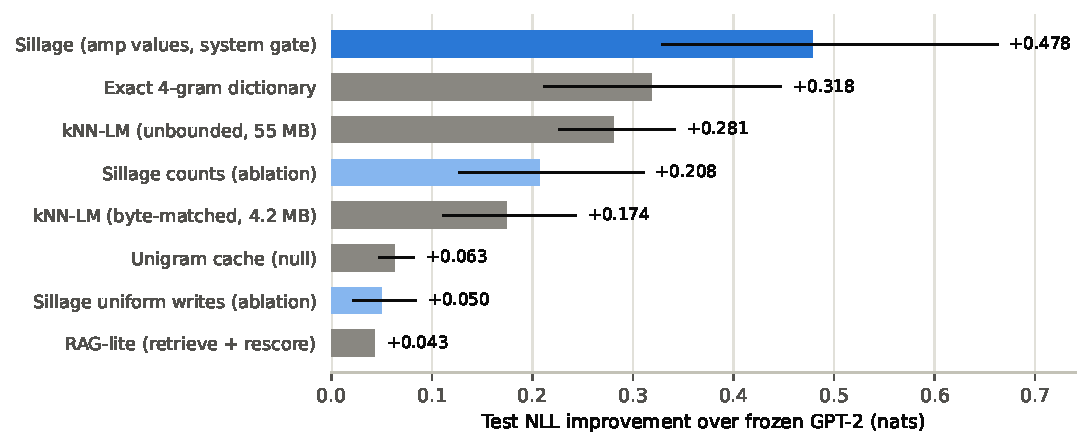
\includegraphics[width=\linewidth]{figs/fig1_main.pdf}
\caption{Test NLL improvement over frozen GPT-2 on \textsc{Manuscripts} (36k tokens of novel technical text; base PPL 31.2). Whiskers: 95\% block-bootstrap CIs (single seed; the \sillage{} headline replicates at $+0.486\pm0.005$ over 5 hypervector seeds). Blue: \sillage{} variants; gray: baselines. \sillage{} uses 4.2\,MB of fixed storage; unbounded kNN-LM uses 55\,MB and grows.}
\label{fig:main}
\end{figure}

\begin{table}[t]
\centering\small
\caption{Test $\dnll$ (nats) over the frozen LM; 95\% block-bootstrap CIs; memory at end of stream. \sillage{} rows on \textsc{Manuscripts}: mean$\,\pm\,$SEM over 5 hypervector seeds.}
\label{tab:main}
\begin{tabular}{@{}lccc@{}}
\toprule
& \textsc{Manuscripts} & \textsc{Einstein} & \textsc{Alice}\\
\midrule
\sillage{} (amp, system gate, $n{=}4$) --- 4.2\,MB & $\mathbf{+0.486 \pm 0.005}$ & $+0.018$ & $+0.007$\\
\sillage{} ($n{=}2{+}4{+}8$) --- 12.6\,MB & --- & $\mathbf{+0.035 \pm 0.000}$ & $+0.017 \pm 0.000$\\
kNN-LM unbounded (55--62\,MB) & $+0.281$ \ci{0.227}{0.341} & $+0.033$ \ci{0.027}{0.037} & $\mathbf{+0.022}$ \ci{0.019}{0.025}\\
kNN-LM @ 4.2\,MB & $+0.174$ \ci{0.112}{0.243} & $+0.018$ \ci{0.014}{0.022} & $+0.006$ \ci{0.003}{0.009}\\
Exact 4-gram dictionary & $+0.318$ \ci{0.212}{0.447} & $+0.006$ \ci{0.002}{0.012} & $-0.004$ (harmful)\\
RAG-lite (interpolated) & $+0.043$ & $+0.010$ & $+0.008$\\
Unigram cache (null) & $+0.063$ \ci{0.048}{0.082} & $+0.005$ & $-0.003$\\
\bottomrule
\end{tabular}
\end{table}

Figure~\ref{fig:main} and Table~\ref{tab:main} give the main comparison. On the novel, repetitive \textsc{Manuscripts} stream, \sillage{} reaches $+0.486\pm0.005$ nats (PPL $31.2 \to 19.2$) with 4.2\,MB of fixed storage. The \textbf{paired} comparison against \emph{unbounded} kNN-LM --- $+0.198$ nats in \sillage's favor, CI95 $[+0.091, +0.325]$, $P(\text{\sillage{} better})=1.000$ --- is the headline: a constant-size, gradient-free matrix outperforms the growing exact datastore it was designed to approximate, on the stream type it targets. The exact 4-gram dictionary is a strong competitor there ($+0.318$) but is brittle off-domain (harmful on \textsc{Alice}) and grows $O(N)$; \sillage{} beats it everywhere while never hurting. On the low-repetition classics all methods are within a few hundredths of a nat; the multi-scale key doubles \sillage's gain and overtakes unbounded kNN-LM on \textsc{Einstein} ($+0.035$ vs $+0.033$, at $1/5$th the memory), while \textsc{Alice} remains kNN's best case.

\subsection{Replication on a second model}\label{sec:qwen}

\begin{table}[t]
\centering\small
\caption{Replication on frozen Qwen3-0.6B (vocabulary 151{,}936; hidden size 1024). Test $\dnll$ (nats), 95\% block-bootstrap CIs on the headline column; single hypervector seed.}
\label{tab:qwen}
\begin{tabular}{@{}lccc@{}}
\toprule
& \textsc{Manuscripts} & \textsc{Einstein} & \textsc{Alice}\\
& (base PPL 14.9) & (base PPL 13.0) & (base PPL 20.8)\\
\midrule
\sillage{} (amp, system gate, $n{=}4$) --- 4.2\,MB & $+0.258$ \ci{0.160}{0.373} & $+0.005$ & $+0.002$\\
\sillage{} ($n{=}2{+}4{+}8$) --- 12.6\,MB & --- & $+0.014$ & $+0.009$\\
\sillage{} counts (ablation) & $+0.231$ & $+0.003$ & $+0.002$\\
kNN-LM unbounded (68--82\,MB) & $\mathbf{+0.273}$ \ci{0.231}{0.321} & $\mathbf{+0.070}$ & $\mathbf{+0.083}$\\
kNN-LM @ 4.2\,MB & $+0.184$ & $+0.029$ & $+0.042$\\
Exact 4-gram dictionary & $+0.151$ & $-0.007$ (harmful) & $-0.013$ (harmful)\\
Unigram cache (null) & $+0.026$ & $+0.008$ & $+0.014$\\
\bottomrule
\end{tabular}
\end{table}

Table~\ref{tab:qwen} repeats the full protocol on Qwen3-0.6B, a modern model whose base perplexity on \textsc{Manuscripts} is half GPT-2's (14.9 vs 31.2) --- less headroom and a harder test. Every internal ordering replicates: amplitudes beat counts, \sillage{} beats the byte-matched kNN-LM, the dictionary is again strong on the repetitive stream and again \emph{harmful} on both classics, and the null cache is small. On \textsc{Manuscripts}, \sillage{} ($+0.258$, 4.2\,MB fixed) is statistically indistinguishable from \emph{unbounded} kNN-LM ($+0.273$, $\sim$68\,MB): the paired block-bootstrap difference is $0.015$ nats (nominally favoring kNN-LM), CI95 $[-0.081, +0.060]$ --- parity at one-sixteenth the memory, where GPT-2 gave \sillage{} an outright win. On the classics, the stronger model's 1024-dimensional representations make semantic retrieval decisively better (kNN $+0.070$/$+0.083$ vs multi-scale \sillage{} $+0.014$/$+0.009$): the regime boundary of \S\ref{sec:scaling} is \emph{sharper} on the stronger model, because what \sillage{} lacks --- soft semantic matching --- is exactly what improves with model quality.

\subsection{Downstream task: content-token recall after one reading}\label{sec:cloze}

Perplexity gains only matter if they surface in behavior. We therefore evaluate \emph{content-token recall}: at up to 2{,}000 automatically selected test positions whose target is a content word (leading-space alphabetic piece, $\ge 5$ characters, token type already seen $\ge 2$ times earlier in the stream), each system predicts the next token by greedy argmax. Every system uses the interpolation settings tuned on that stream's dev split \emph{for perplexity} --- no task-specific tuning --- and candidates are the union of the base model's and the memory's top-128 (Appendix~\ref{app:params}).

\begin{table}[t]
\centering\small
\caption{Content-token recall (top-1 accuracy, \%; Wilson 95\% CIs; 2{,}000 items per row). McNemar column: items fixed\,:\,broken by \sillage{} relative to the frozen model.}
\label{tab:cloze}
\begin{tabular}{@{}llcccc@{}}
\toprule
model & stream & frozen & $+$kNN-LM & $+$\sillage{} & fixed\,:\,broken\\
\midrule
GPT-2 & \textsc{Manuscripts} & 11.3 \ci{10.0}{12.8} & 11.3 \ci{9.9}{12.7} & $\mathbf{23.7}$ \ci{21.8}{25.6} & $261:14$\\
Qwen3-0.6B & \textsc{Manuscripts} & 19.7 \ci{18.0}{21.5} & 19.9 \ci{18.2}{21.7} & $\mathbf{24.0}$ \ci{22.2}{25.9} & $97:10$\\
GPT-2 & \textsc{Tolstoy} (500k) & 15.0 \ci{13.5}{16.6} & 15.2 \ci{13.7}{16.8} & 15.0 \ci{13.5}{16.6} & $0:1$\\
\bottomrule
\end{tabular}
\end{table}

\begin{figure}[t]
\centering
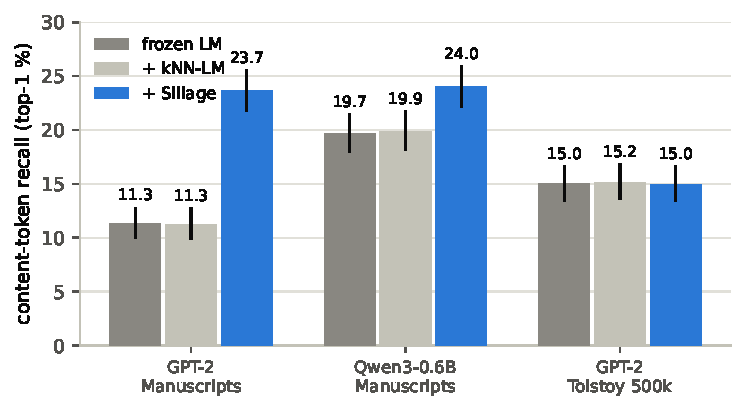
\includegraphics[width=0.7\linewidth]{figs/fig4_downstream.pdf}
\caption{Content-token recall (top-1, \%) with Wilson 95\% CIs. \sillage{} converts its perplexity gains into behavior; kNN-LM, tuned identically, does not move the argmax; and where \sillage{} has no perplexity gain (\textsc{Tolstoy}), it claims no recall gain either.}
\label{fig:cloze}
\end{figure}

Table~\ref{tab:cloze} and Figure~\ref{fig:cloze}: after a single reading pass of the novel technical stream, \sillage{} \textbf{more than doubles} GPT-2's recall of recurring content tokens ($11.3\% \to 23.7\%$, disjoint CIs; it fixes 261 items and breaks 14) and lifts the much stronger Qwen3 baseline from $19.7\%$ to $24.0\%$ ($97:10$). On the recurring-term subset (type seen $\ge 5$ times) the pattern is identical ($13.2 \to 23.7$ and $22.2 \to 26.0$). Two honest observations. First, kNN-LM --- despite its perplexity gains --- leaves top-1 accuracy unchanged everywhere: its tuned interpolation weight ($\lambda = 0.05$--$0.1$) almost never flips the argmax, whereas the amplitude memory's earned trust ($\lambda = 0.3$) does; NLL improvements do not automatically convert to behavioral ones. Second, the effect is dose-responsive: on \textsc{Tolstoy}, where \sillage's perplexity gain is marginal ($+0.005$ nats), its recall gain is exactly zero --- no unexplained transfer, no artifact. Appendix~\ref{app:examples} shows representative completions.

\subsection{Mechanism attribution}\label{sec:mech}

\begin{figure}[t]
\centering
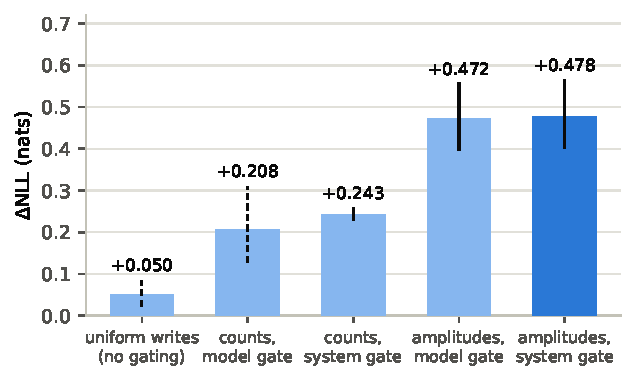
\includegraphics[width=0.62\linewidth]{figs/fig3_mechanisms.pdf}
\caption{Factorial attribution on \textsc{Manuscripts} (GPT-2): value encoding $\times$ write gate, plus the no-gating ablation. Whiskers: \emph{paired} 95\% block-bootstrap CIs against the count/model-gate control, recentred on each bar (solid) --- the estimator that matches the comparison the figure makes; marginal CIs for the control and the no-gating ablation (dashed). Amplitude values are the dominant factor; every effect is positive in all 5 hypervector seeds.}
\label{fig:mech}
\end{figure}

Figure~\ref{fig:mech} decomposes the gain. \textbf{Amplitude values} contribute $+0.265$ nats over counts (paired, $P=1.000$; replicated $+0.283\pm0.005$, positive in 5/5 seeds) --- Proposition~\ref{prop:amp} in action, with the predicted diagnostic that the tuned interpolation weight rises from $0.05$ to $0.3$--$0.4$. The \textbf{system gate} adds a small, certain, free improvement ($+0.036$, $P=1.000$). \textbf{Surprise gating} itself quadruples the gain of uniform writes at equal plasticity budget ($+0.203$ vs $+0.050$ for the count variant), with a consistent sign on all three streams. The \textbf{multi-scale key} is the lever for low-repetition text ($+0.019\pm0.000$ on \textsc{Einstein}, $+0.011\pm0.000$ on \textsc{Alice}, all seeds positive) and is redundant on the highly repetitive stream. Selected hyperparameters are stable across seeds (softmax $\beta = 40$--$80$, $\lambda = 0.3$--$0.4$, abstention at the 75th confidence percentile).

\subsection{Scaling to 500k tokens}\label{sec:scaling}

\begin{figure}[t]
\centering
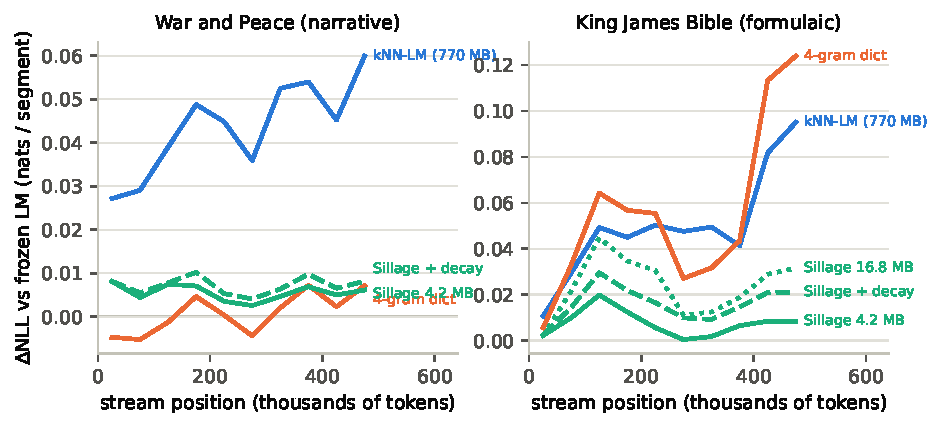
\includegraphics[width=\linewidth]{figs/fig2_scaling.pdf}
\caption{Per-segment $\dnll$ (50k-token bins) on the two 500k streams (GPT-2). Unbounded stores (kNN-LM, dictionary) grow with position; the fixed 4.2\,MB \sillage{} saturates on \textsc{Bible} (rise, collapse near 300k) unless it forgets (dashed) or is sized up (dotted, 16.8\,MB).}
\label{fig:scaling}
\end{figure}

\begin{table}[t]
\centering\small
\caption{500k-token streams: test $\dnll$ (nats) and memory. The fixed matrix operates at $\sim$0.5 writes/parameter and saturates; forgetting and capacity are the two remedies.}
\label{tab:scaling}
\begin{tabular}{@{}lccc@{}}
\toprule
& \textsc{Tolstoy} & \textsc{Bible} & memory\\
\midrule
kNN-LM unbounded & $\mathbf{+0.048}$ \ci{0.045}{0.050} & $+0.058$ \ci{0.053}{0.062} & 770\,MB, $O(N)$\\
Exact 4-gram dictionary & $+0.002$ & $\mathbf{+0.065}$ \ci{0.056}{0.074} & 6--13\,MB, $O(N)$\\
\sillage{} amp, 4.2\,MB & $+0.005$ & $+0.008$ & fixed\\
\sillage{} amp $+$ decay (half-life 100k) & $+0.007$ & $+0.018$ \ci{0.016}{0.020} & fixed\\
\sillage{} counts (control) & --- & $+0.010$ \ci{0.008}{0.012} & fixed\\
\sillage{} amp, $D_K{=}16384$ & --- & $+0.027$ \ci{0.023}{0.030} & 16.8\,MB fixed\\
Unigram cache & $+0.005$ & $-0.003$ & 0.2\,MB\\
\bottomrule
\end{tabular}
\end{table}

Figure~\ref{fig:scaling} and Table~\ref{tab:scaling} map the long-horizon regime. Three findings. \textbf{(i) A fixed memory must forget at long horizons}: on \textsc{Bible}, \sillage's per-segment gain rises to $+0.020$ by 150k tokens, collapses to $\approx 0$ near 300k as the matrix fills, and only partially recovers; the decayed variant instead sustains $+0.010$--$0.030$ across the entire stream ($2.3\times$ the total gain). \textbf{(ii) Capacity is a sizing knob, not a wall}: quadrupling $D_K$ (16.8\,MB; $0.5 \to 0.12$ writes/parameter) raises the no-decay gain from $+0.008$ to $+0.027$ --- more than the small matrix achieves even with forgetting --- and its per-segment gains no longer collapse. At 16.8\,MB, \sillage{} reaches 46\% of unbounded kNN's gain at 2\% of its storage. Notably, at saturation the amplitude advantage vanishes (counts $+0.010 \approx$ amplitudes $+0.008$ without decay): in that regime interference, not encoding, binds. \textbf{(iii) The boundary is honest}: on long, low-repetition narrative, soft semantic retrieval over an unbounded store wins ($+0.048$ vs $+0.007$); \sillage's domain is bounded-memory streaming over structured, novel, or byte-constrained settings --- the on-device and continual regime.

\section{Discussion}

\textbf{Why amplitudes work.} A superposed count vector is dominated by frequent successors; rare continuations drown in crosstalk. Storing $\sqrt{\text{mass}}$ compresses the coefficient range (Proposition~\ref{prop:amp}), and the tuner's behavior confirms the mechanism: it trusts the amplitude memory six times more. The same square-root geometry underlies classical affinity measures between distributions \cite{bhatta43,jebara,rootsift}; its role here --- conditioning a \emph{superposed Hebbian store} --- appears to be new.

\textbf{Relation to learned test-time memories.} \sillage{} reproduces, gradient-free, the ingredient list of Titans and its relatives \cite{titans,ttt,ttr}: a bounded associative store, surprise-proportional writing, forgetting. The trade is explicit: those systems learn their keys and can generalize semantically; \sillage's keys are surface $n$-grams, which is why it dominates on repetitive novel text and cedes long narrative to kNN. A hybrid --- learned keys, amplitude values, log-loss gating --- is the natural meeting point.

\textbf{A memory hierarchy.} The results sketch an architecture rather than a single module: a fast fixed-size amplitude memory for the immediate stream; consolidation, arbitrated by the same surprise signal, into an exact cold store (the dictionary that wins on formulaic text at scale); and unbounded semantic retrieval as the slowest, largest tier. The three systems this paper benchmarks against each other are, in that reading, tiers of one memory system.

\textbf{A biological reading.} The full loop --- Hebbian rank-1 writes, a global scalar gate equal to the model's own prediction loss, sublinear (square-root) synaptic accumulation, slow decay --- is implementable in the three-factor vocabulary of neuromodulated plasticity \cite{fremaux,izhikevich} with no error transport of any kind.

\section{Limitations}

Two frozen LMs (124M and 0.6B) and CPU-scale streams; perplexity plus one downstream task (no reasoning benchmarks); 500k streams scored at stride 4; classic corpora partially memorized by the base models (\textsc{Manuscripts} is the clean case); the 40k-token cap is applied per tokenizer, so on the two Gutenberg classics GPT-2 and Qwen3 read different spans of the same text (Qwen3's denser tokenizer covers more; \textsc{Manuscripts} is content-identical for both) --- within-model orderings are unaffected, but cross-model comparisons on those two streams compare slightly different content; the system gate's write-time normalization scales with vocabulary size and was replaced by the model gate at 500k; $n$-gram keys capture surface repetition only --- the measured failure of hidden-state keys (Appendix~\ref{app:negative}) means semantic generalization is currently delegated entirely to the frozen LM; hyperparameters are tuned on the dev prefix of each stream (standard streaming practice; cross-stream transfer of tuned settings is future work).

\section{Conclusion}

A single Hebbian matrix --- keys by sliding vector-symbolic $n$-gram binding, values by square-root amplitudes, writes gated by the model's own surprise --- gives a frozen language model a 4.2\,MB, gradient-free, constant-size episodic memory that beats retrieval-augmented rescoring everywhere tested, beats an unbounded kNN-LM on novel repetitive text with certainty (paired $P = 1.000$) at $1/13$th the memory, replicates across two model families, improves downstream recall of recurring technical terms after a single reading, and degrades gracefully where exact caches turn harmful. Its three design choices are separately attributed and replicated, and each traces to a principle: compositional binding for selectivity, square-root encoding for superposition conditioning, and free-energy gating for write allocation. Its failure modes are equally explicit --- saturation at $\sim$0.5 writes per parameter (with forgetting and sizing as quantified remedies) and blindness to soft semantic matches. The natural next stage is the memory hierarchy the results already sketch, and the search for gradient-free \emph{semantic} keys to close the remaining gap.

\appendix

\section{Negative result: hidden states are not Hebbian keys}\label{app:negative}

Centered-cosine similarity between GPT-2 final hidden states at random position pairs on \textsc{Manuscripts} has mean $0.32$ but \emph{95th percentile $0.94$} (archived in \texttt{results/semantic\_diag\_bhd.json}): the overlap tail is fatal to a linear superposition readout, which mixes thousands of near-duplicate keys. Sparse top-$w$ sign projections, dense normalized projections, and hybrid semantic$+$$n$-gram keys were all tuned and evaluated; the best semantic-only configuration reaches $+0.040$ on \textsc{Manuscripts} (vs.\ $+0.486$ for $n$-gram keys) and is \emph{harmful} on \textsc{Einstein} ($-0.002$). Selectivity, not dimensionality, is the binding constraint: kNN survives the same geometry only because hard top-$k$ retrieval is a nonlinearity that outer-product memories do not possess.

\section{Downstream task examples}\label{app:examples}

Representative content-token completions on \textsc{Manuscripts} (GPT-2) where the augmented model is correct and the frozen model is not. Contexts are abbreviated; \verb|/| marks a line break in the source.

\begin{center}\small
\begin{tabular}{@{}p{7.6cm}lll@{}}
\toprule
context (end) & truth & frozen & $+$\sillage{}\\
\midrule
\ldots substituting KL divergence with cosine & distance & . & distance\\
\ldots cosine distance in HDC & spaces & . & spaces\\
\ldots that an STDP-modulated agent & using & can & using\\
\ldots gradient descent --- faces three / fundamental & limitations & challenges & limitations\\
\ldots Neuromorphic Computing, AGI, Continual & Learning & / & Learning\\
\ldots artificial intelligence --- transformer-based & large & learning & large\\
\bottomrule
\end{tabular}
\end{center}

The pattern is characteristic: the frozen model produces a generic continuation (punctuation, a common adjective), while the memory recalls the specific recurring term of the document being read.

\section{Hyperparameters and reproduction}\label{app:params}

Memory: $D_K = 4096$ per scale, $D_V = 256$, fp32; token hypervectors regenerated from seeds. Readout grid: softmax $\beta \in \{2,5,10,20,40,80,160\}$ or quadratic; $\lambda \in \{0.02,\dots,0.85\}$ (10 values); abstention threshold $\in \{\text{none}, q_{25}, q_{50}, q_{75}\}$ of the dev confidence (maximum normalized score). Gate cap 5 nats; system gate mixes $\tilde\lambda = 0.2$ at $\beta = 20$. Decay (500k only): half-life 100k tokens. kNN: $k \in \{8,16,32\}$, $\tau \in \{0.5,1,3\}$, L2 over unit-normalized final hidden states. RAG: 128-token chunks, top-1 by mean-pooled cosine, 512-token local context, 256-token rescored blocks. Splits: dev $=$ first 20\% of positions. Hypervector seeds $\{11,22,33,44,55\}$ ($+7001$ for single-seed runs); all data and protocol seeds are fixed in code. Grid-edge check: on the Qwen \textsc{Manuscripts} stream the tuner selected the top of the $\beta$ grid ($\beta{=}160$); extending the grid to $\{320, 640\}$ changed the test result by $<0.001$ nats, so no gain is left at the boundary. Downstream task: test-region positions whose target decodes to a leading-space alphabetic piece of $\ge 5$ characters with token type seen $\ge 2$ times earlier; up to 2000 items; predictions by greedy argmax over the union of the base model's and the memory's top-128 candidates, using each stream's perplexity-tuned interpolation settings (no task-specific tuning).

The complete experimental pipeline (corpus preparation, one frozen-LM pass per stream, every baseline and ablation, statistics, and figures) is released as documented Python scripts; every number and figure in this paper regenerates from them with fixed seeds.

\begin{thebibliography}{19}\small

\bibitem{khandelwal2020} U.~Khandelwal, O.~Levy, D.~Jurafsky, L.~Zettlemoyer, M.~Lewis.
Generalization through memorization: Nearest neighbor language models. \emph{ICLR}, 2020.

\bibitem{grave} E.~Grave, A.~Joulin, N.~Usunier.
Improving neural language models with a continuous cache. \emph{ICLR}, 2017.

\bibitem{gpt2} A.~Radford, J.~Wu, R.~Child, D.~Luan, D.~Amodei, I.~Sutskever.
Language models are unsupervised multitask learners. OpenAI Technical Report, 2019.

\bibitem{retro} S.~Borgeaud et al.
Improving language models by retrieving from trillions of tokens. \emph{ICML}, 2022.

\bibitem{memtrans} Y.~Wu, M.~N.~Rabe, D.~Hutchins, C.~Szegedy.
Memorizing Transformers. \emph{ICLR}, 2022.

\bibitem{hopfield} H.~Ramsauer et al.
Hopfield networks is all you need. \emph{ICLR}, 2021.

\bibitem{ttt} Y.~Sun et al.
Learning to (learn at test time): RNNs with expressive hidden states. arXiv:2407.04620, 2024.

\bibitem{titans} A.~Behrouz, P.~Zhong, V.~Mirrokni.
Titans: Learning to memorize at test time. arXiv:2501.00663, 2025.

\bibitem{ttr} K.~A.~Wang, J.~Shi, E.~B.~Fox.
Test-time regression: A unifying framework for designing sequence models with associative memory. arXiv:2501.12352, 2025.

\bibitem{nested} A.~Behrouz, M.~Razaviyayn, P.~Zhong, V.~Mirrokni.
Nested learning: The illusion of deep learning architectures. arXiv:2512.24695, 2025.

\bibitem{kanerva} P.~Kanerva.
Hyperdimensional computing: An introduction to computing in distributed representation with high-dimensional random vectors. \emph{Cognitive Computation}, 1(2):139--159, 2009.

\bibitem{plate} T.~A.~Plate.
Holographic reduced representations. \emph{IEEE Transactions on Neural Networks}, 6(3):623--641, 1995.

\bibitem{kleyko} D.~Kleyko, D.~A.~Rachkovskij, E.~Osipov, A.~Rahimi.
A survey on hyperdimensional computing aka vector symbolic architectures, Part~I. \emph{ACM Computing Surveys}, 55(6):1--40, 2023.

\bibitem{bhatta43} A.~Bhattacharyya.
On a measure of divergence between two statistical populations defined by their probability distributions. \emph{Bulletin of the Calcutta Mathematical Society}, 35:99--109, 1943.

\bibitem{jebara} T.~Jebara, R.~Kondor.
Bhattacharyya and expected likelihood kernels. \emph{COLT}, LNCS 2777:57--71, 2003.

\bibitem{rootsift} R.~Arandjelovi\'c, A.~Zisserman.
Three things everyone should know to improve object retrieval. \emph{CVPR}, 2911--2918, 2012.

\bibitem{fremaux} N.~Fr\'emaux, W.~Gerstner.
Neuromodulated spike-timing-dependent plasticity, and theory of three-factor learning rules. \emph{Frontiers in Neural Circuits}, 9:85, 2016.

\bibitem{izhikevich} E.~M.~Izhikevich.
Solving the distal reward problem through linkage of STDP and dopamine signaling. \emph{Cerebral Cortex}, 17(10):2443--2452, 2007.

\end{thebibliography}

\end{document}
